\section{SCL object model}
\label{sec:ch-scl--SCL-object-model}
As explained in the section \ref{sec:ch-scl--SCL-definition}, 
the SCL describes the SAS by modelling objects.
The standard IEC 61850-6 \cite{IEC61850-6:2004} object model 
structure and constraints are described in terms of the 
\gls{XSD}.

The \gls{XSD} of the \gls{SCL} are structured as depicted 
in the figure \href{fig:pdf-SCL-uml-deept2}. 

\begin{center}
	\begin{figure}
	  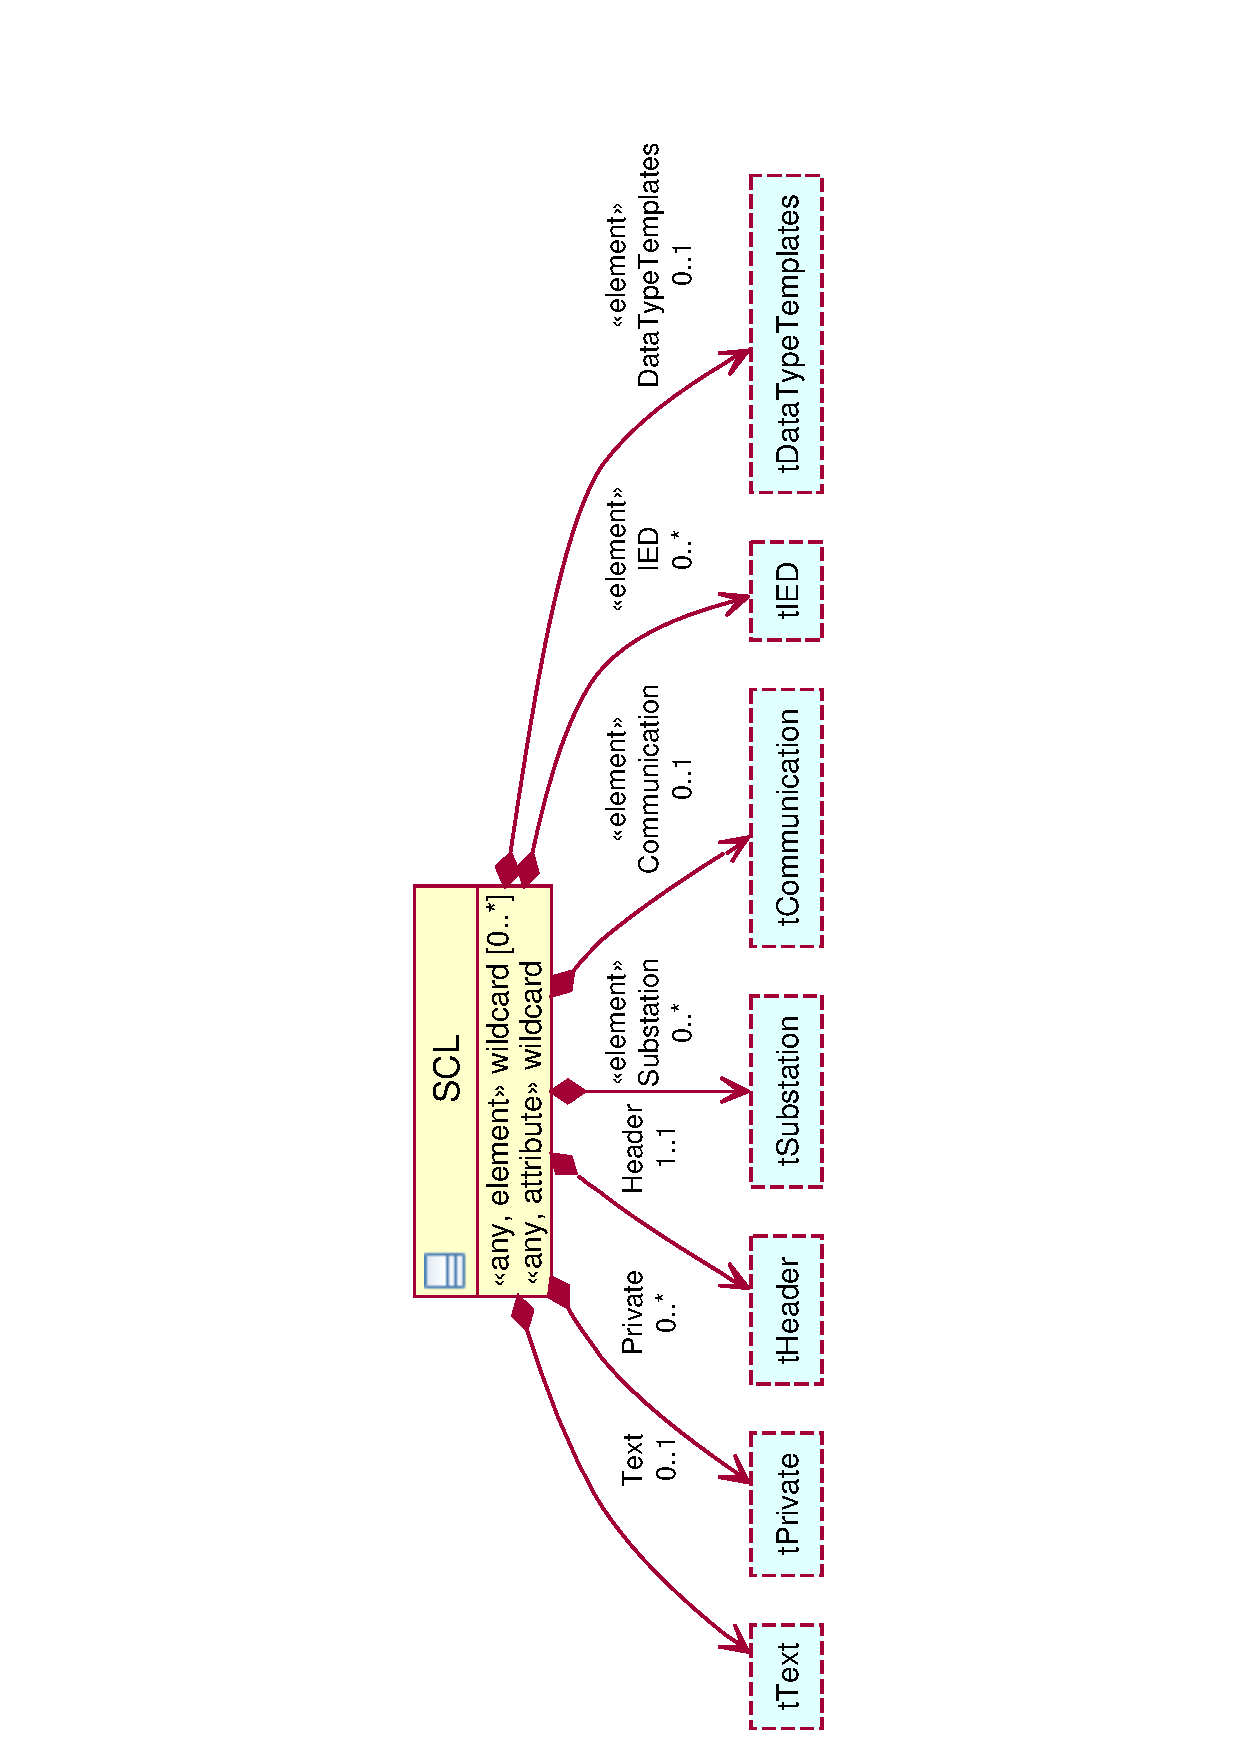
\includegraphics[
						angle=-90,	  
	  					width=1.0\textwidth 
	  				   ]{chapters/ch-scl/figures/SCL-uml-Deept2}
	  \caption{SCL object model}  
	  \label{fig:pdf-SCL-uml-deept2}
	\end{figure}
\end{center}
 
%\begin{landscape}
%\end{landscape}


Basically, it is composed by: 
\todo[color=green!40]{61850, parte6, cl6.1, \textparagraph 5}



\begin{itemize}
  \item The substation model: the object model of the primary power structure
  		(a instance of tSubstation) with their designations structured according to 
  		IEC 61346-1 \cite{IEC61346-1:1996}. 
  \item The communication model: the object model of the IED 
  		communication system configuration, 
  		i.e.,
  		the the networks, subnetworks, ports informations
  		\todo[color=green!40]{61850, parte6, cl6.1, \textparagraph 5},
  		the communication connection relations of IEDs to 
  		subnetworks, the routing for another subnetworks informations, 
  		and clocks configuration information and locations for 
  		time synchronisation (the gateways are not considered here, 
  		a gateway has to be modelled as another IED)
  		\todo[color=green!40]{61850, parte6, cl6.1, \textparagraph 8}.
  \item The product model: Contains the IEDs objects and their 
  		logical node implementations. 
  \todo[inline]{averiguar la funcion del DataTypeTemplates para agregar aca
  si corresponde}
\end{itemize}

All the structures are derived from differents 
parts depicted in the figure \ref{fig:pdf-SCL-uml-deept2}. 
In this figure, each class represent the top level 
of their structure, e.g., the substation class 
mentioned here has voltage levels, 
connectivity nodes and tranformers.   
Theses classes are completely decoupled 
(the most notable decoupling are the diferentiation of  
Logical node classes on the 
IED -t\gls{LN}- and Substation -t\gls{LNode}- structure), 
allowing the separation of the \gls{SCL} development 
by the differents engineering process 
described in the section \ref{sec:SCL-engineering-parts}.


The \gls{SCL} relationship are based in a 
ring \gls{O-O} architecture between Substation,
IED, Header, Communication, and DataTypeTemplate classes,
and it are based in a hierarchical structure under each of the 
mentioned classes.



\subsection{SCL modelling steps}
\todo[inline]{esta seccion la dejo pendiente,
debo escribirlo con detenimiento para 
que queden en concordancia la 
figura \ref{fig:pdf-SCL-uml-deept2} 
y lo que tengo escrito en esta seccion}

The figure \ref{fig:SCL-development-process} 
show the detailed SAS engineering 
process depicted with 
the autor interpretation of the step 
mentioned in the standard by 
using an \gls{UML} secuence diagram.

The more usual approach for the \gls{SAS} description 
with \gls{SCL} begin with the 
single line drawing process where the 
substation topology are defined using a 
system configurator tool. The system configurator tool, 
described in the section \ref{sec:ch-scl--System-configurator-tool}, 
creates the \gls{SSD} file containing the \glspl{LNode}
and their allocation in the substation. 
The class diagram provided by the author 	 
are based on the \gls{SCL} 
\gls{XSD}['s] of the substation. (figures  
\ref{fig:pdf-SCL-uml-substation-Deept2} and 
\ref{fig:pdf-SCL-uml-substation-Deept2-inherited}).

The \glspl{LNode} objects SCL models 
(from the substation section) is used to map 
the \gls{IED} object model references  
(figure \ref{}
\todo{apuntar a label{fig:pdf-SCL-uml-IED-Deept2}}) 
that describes 
the \gls{IED} objects are used to mapping 
\todo{terminar bien este parrafo\ldots}


\todo[inline]{a este le falta
expandir la clase correspondiente hasta que muestre el transformador }
\begin{figure}
  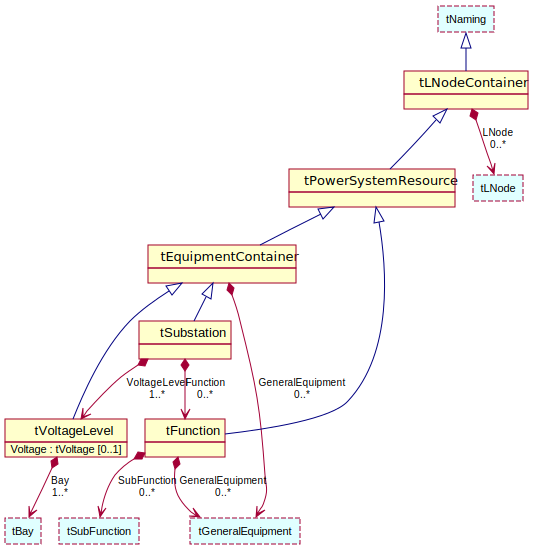
\includegraphics[width=1.0\linewidth]{chapters/ch-scl/figures/SCL-uml-substation-Deept2}
  \caption{SCL Substation class diagram with heritance 
  details} 
  \label{fig:pdf-SCL-uml-substation-Deept2}
\end{figure}


\todo[inline]{a este le valta
  expandir la clase correspondiente hasta que muestre el transformador }
\begin{figure}
  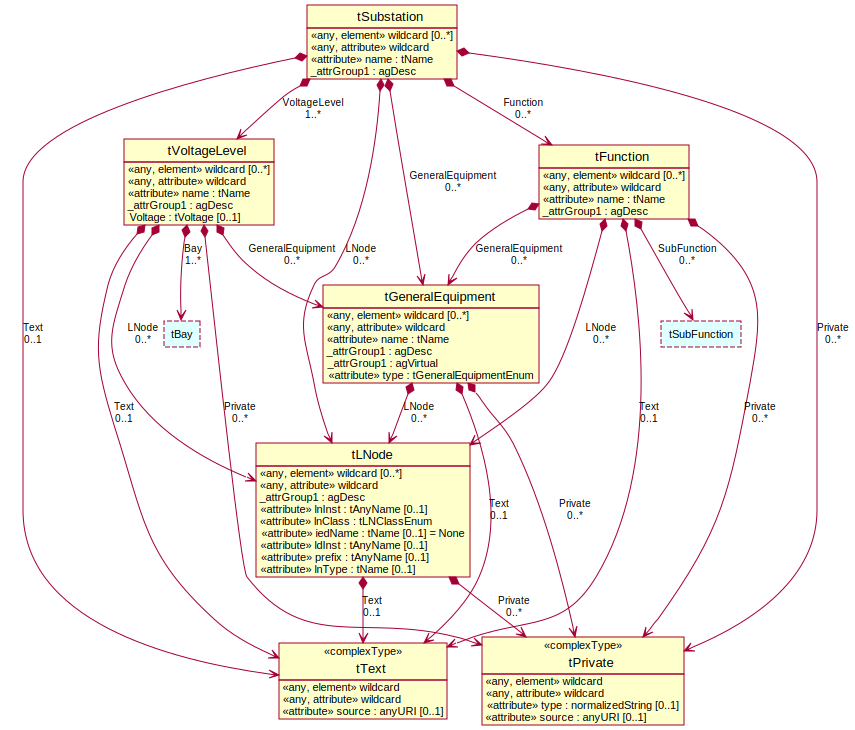
\includegraphics[width=1.0\linewidth]{chapters/ch-scl/figures/SCL-uml-substation-Deept2-inherited}
  \caption{SCL Substation class diagram inherited  }
  \label{fig:pdf-SCL-uml-substation-Deept2-inherited}
\end{figure}


\begin{figure}
  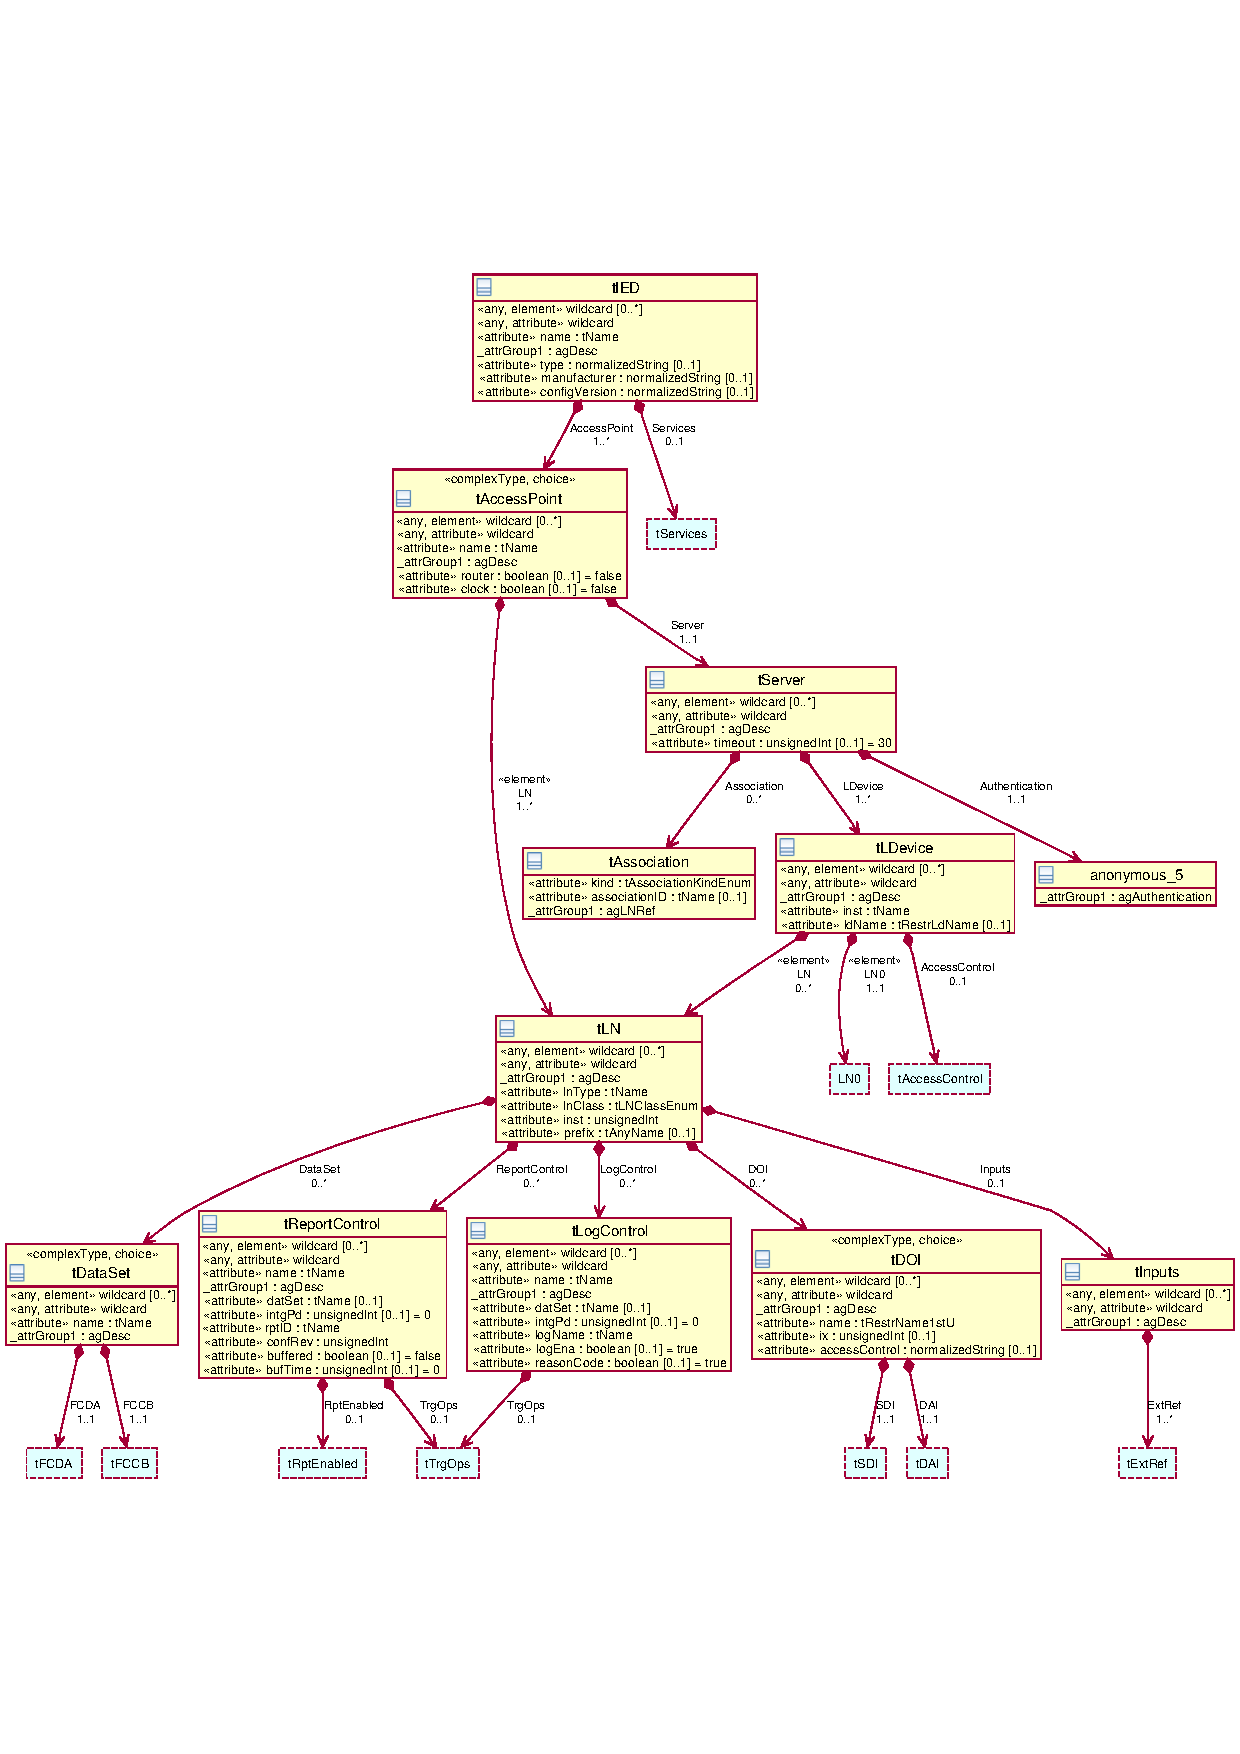
\includegraphics[width=1.0\linewidth]{chapters/ch-scl/figures/SCL-uml-IED-Deept2-inherited}
  \caption{SCL Substation class diagram inherited  }
  \label{fig:pdf-SCL-uml-IED-Deept2-inherited}
\end{figure}

%\begin{figure}
% 
%  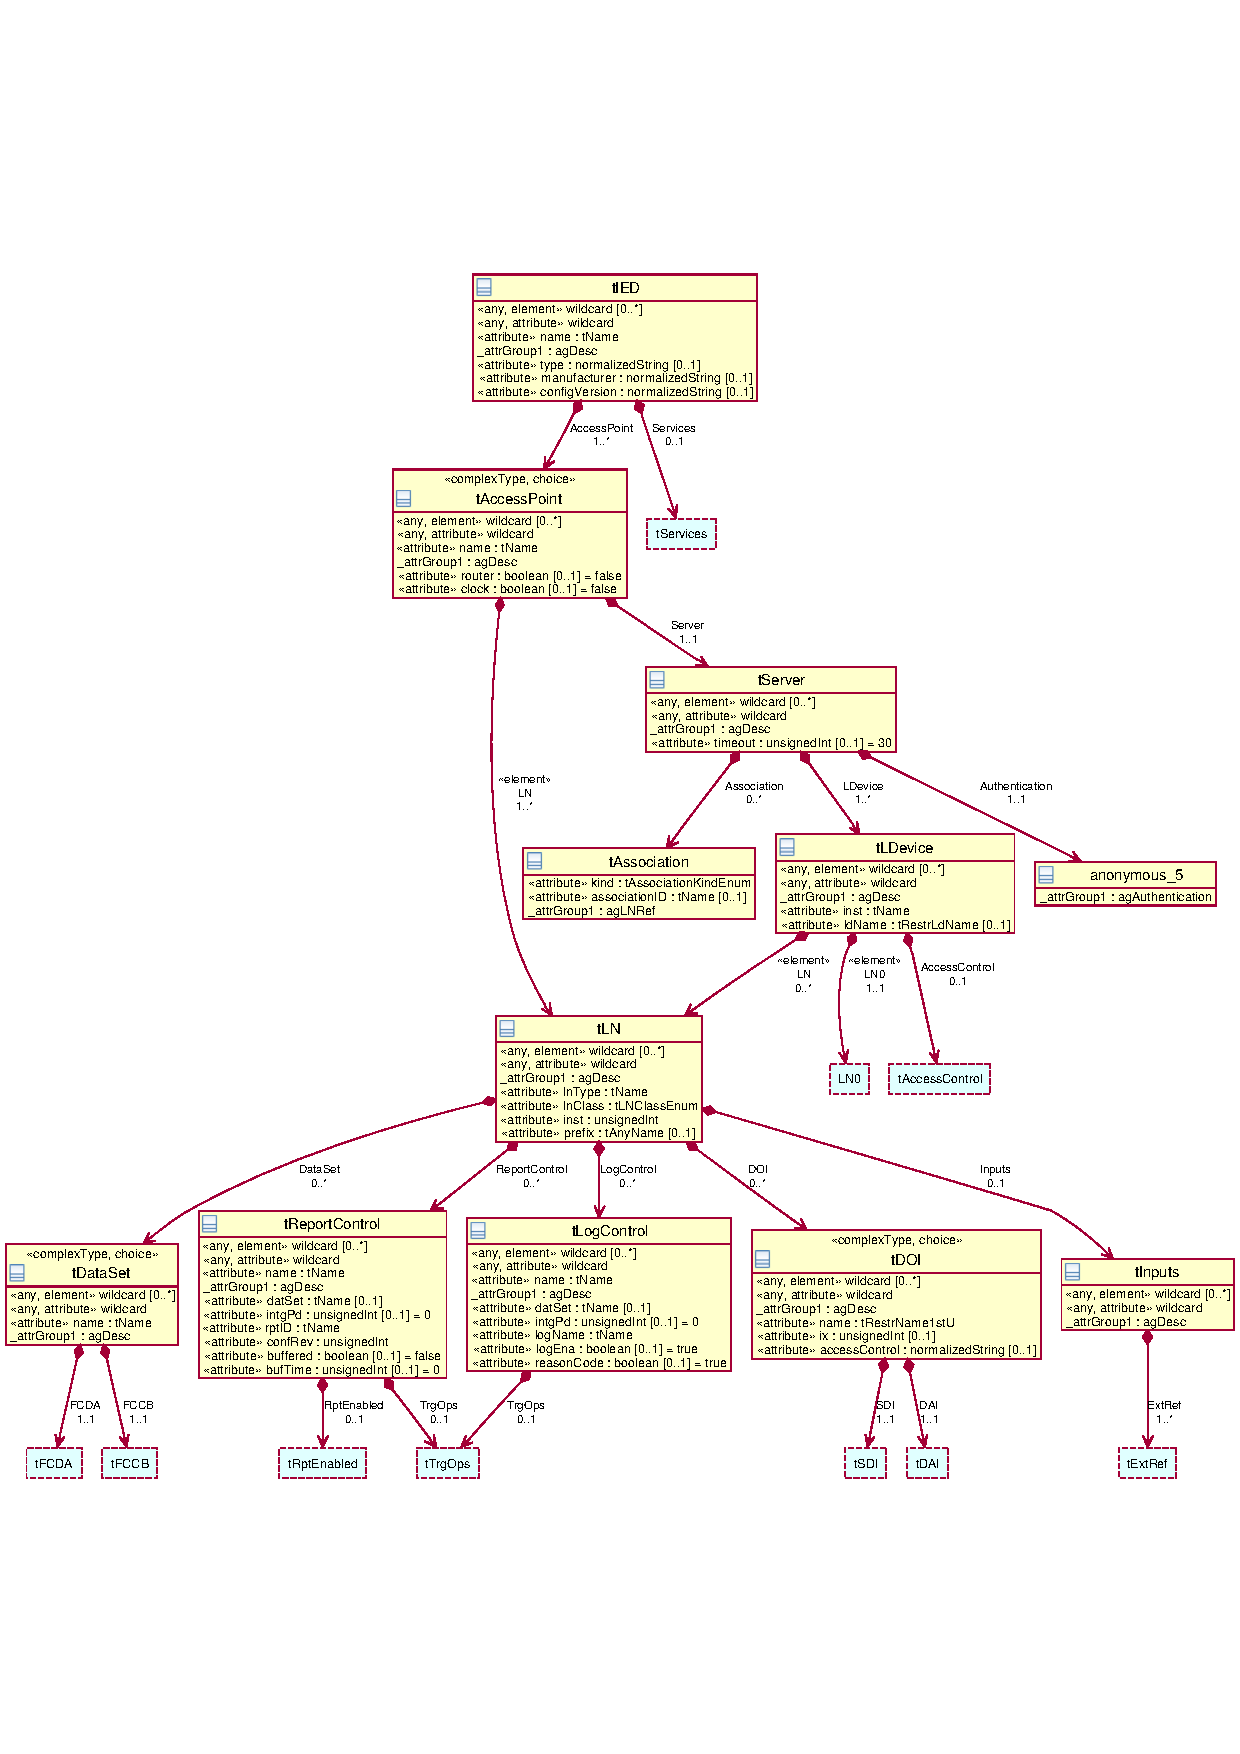
\includegraphics[width=1.0\linewidth]{chapters/ch-scl/figures/SCL-uml-IED-Deept2-inherited}
%  \caption{SCL Substation class diagram inherited  }
%  \label{fig:pdf-SCL-uml-IED-Deept2}
%\end{figure}
\missingfigure[color=green!40]{aqui falta el uml del IED con detalles de
herencia}



\todo[inline]{debo agregar aca la explicacion de los demas modelos
descriptos mediance los XSDs, pues esos tres 
items que menciona la norma son solo los mas
importantes, pero no da para entender y saber leer 
los archivos scl sabiendo solo eso. Los tres items mencionados arriba
son solo la base. Falta principalmente el DATypeTemplate
que corresponden a los objetos a serializar correspondientes 
a las instancias de las clases de la parte 7-x}



\begin{landscape}
	\begin{figure}
	  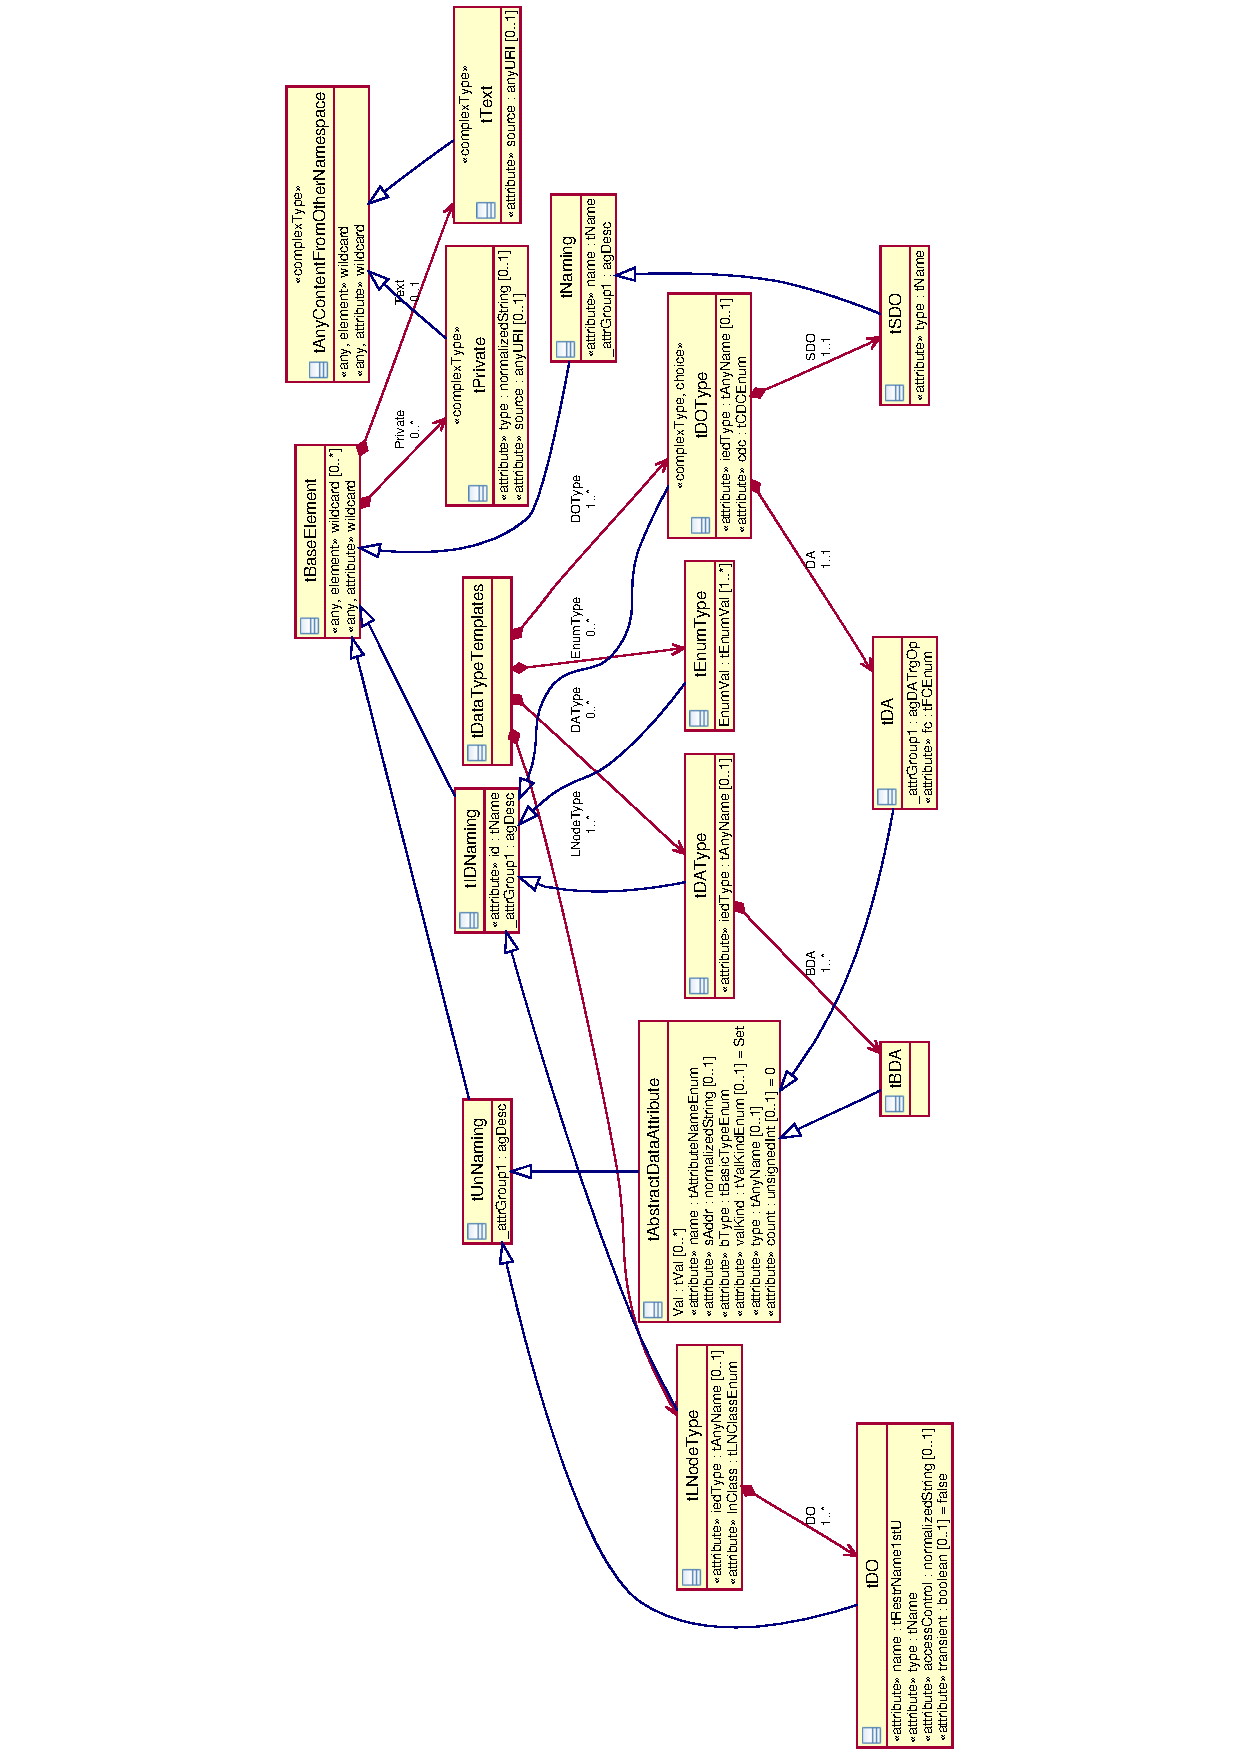
\includegraphics[angle=-90, width=1.0\linewidth]{chapters/ch-scl/figures/SCL-uml-DATypeTemplate-Deept2}
	  \caption{DAType class diagram template with heritance details}  
	  \label{fig:pdf-SCL-uml-DATypeTemplate-Deept2}
	\end{figure}
\end{landscape}

\begin{landscape}
	\begin{figure}
	  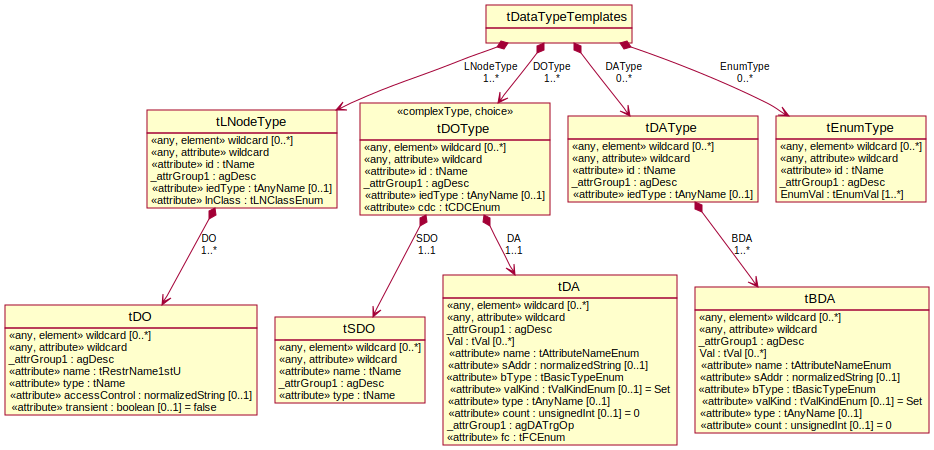
\includegraphics[angle=-90, width=1.0\linewidth]{chapters/ch-scl/figures/SCL-uml-DATypeTemplate-Deept2-inherited}
	  \caption{DAType class diagram template inherited}  
	  \label{fig:pdf-SCL-uml-DATypeTemplate-Deept2-inherited}
	\end{figure}
\end{landscape}

\begin{landscape}
	\begin{figure}
	  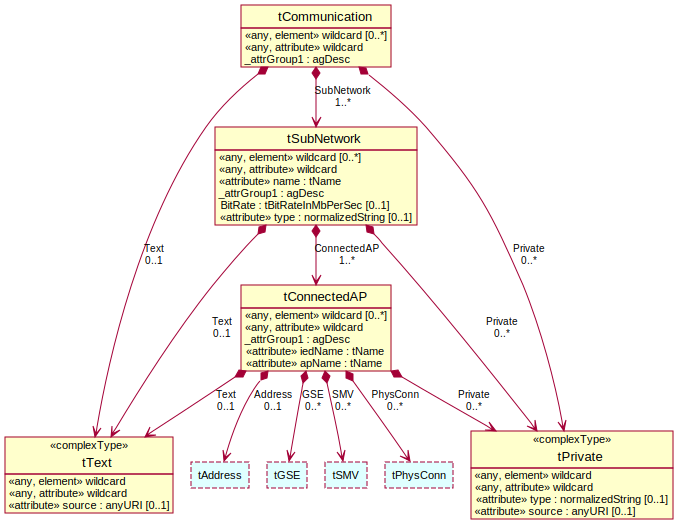
\includegraphics[angle=-90, width=1.0\linewidth]{chapters/ch-scl/figures/SCL-uml-communication-Deept3}
	  \caption{SCL Communication class diagram}  
	  \label{fig:pdf-SCL-uml-communication-Deept3}
	\end{figure}
\end{landscape}


The UML of the 
figure \ref{fig:SCL-uml-Resumen} 
is a resume of
the SCL model, where is evident the 
key importance of the Logical Node for  
the information topology description (see 
the composition of the Substation 
class). The Logical Node is  
the transition object to 
connect the diferent structures of the SAS 
\todo[color=green!40]{61850, parte6, cl6.1, \textparagraph 9} 
that are defined by IEC 61341-1 \cite{IEC61346-1:1996}.


\begin{landscape}

\begin{figure}
  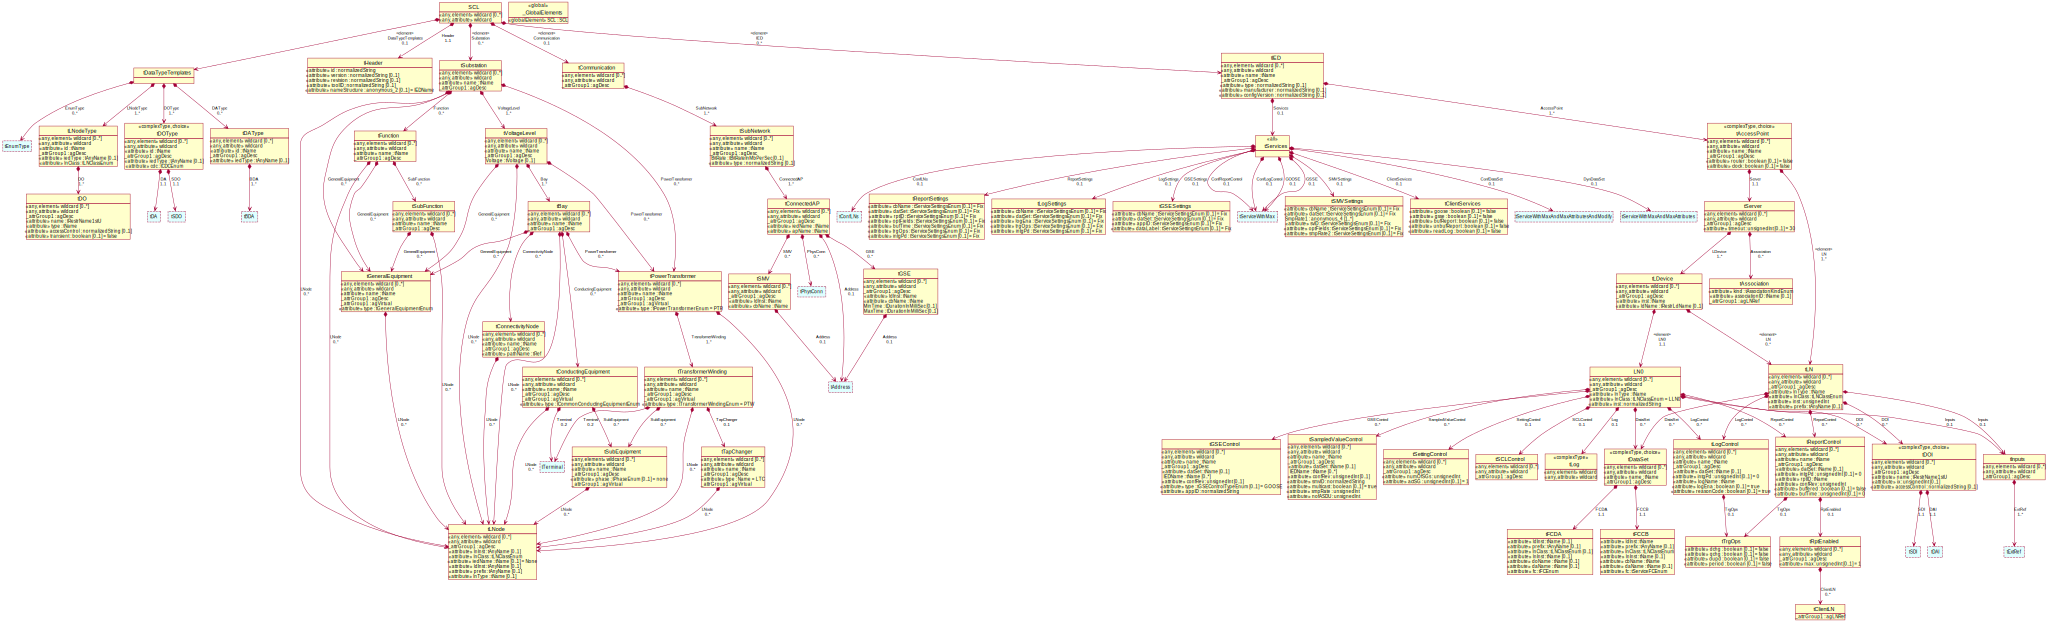
\includegraphics[angle=-90,
  width=1.0\linewidth]{chapters/ch-scl/figures/SCL-uml-Resumen-inherited}
  \caption{Resume of SCL shema represented by a UML class diagram}
  \label{fig:SCL-uml-Resumen}
\end{figure}
\end{landscape}
